% !TeX encoding = UTF-8
% !TeX spellcheck = pl_PL
\documentclass{article}
\newcommand\tab[1][1cm]{\hspace*{#1}}
\usepackage[]{polski}
\usepackage[utf8]{inputenc}
\usepackage{graphicx}
\usepackage{float}
\usepackage{amsmath}
\usepackage{geometry}
 
\usepackage{listings}
\usepackage{color, colortbl}
\usepackage{hyperref}

\usepackage{multirow}
\usepackage{pdfpages}


\definecolor{codegreen}{rgb}{0,0.6,0}
\definecolor{codegray}{rgb}{0.5,0.5,0.5}
\definecolor{codepurple}{rgb}{0.58,0,0.82}
\definecolor{backcolour}{rgb}{0.95,0.95,0.92}

\lstdefinestyle{mystyle}{
	backgroundcolor=\color{backcolour},   
	commentstyle=\color{black},
	keywordstyle=\color{blue},
	numberstyle=\tiny\color{codegray},
	stringstyle=\color{codepurple},
	basicstyle=\footnotesize,
	breakatwhitespace=false,         
	breaklines=true,                 
	captionpos=b,                    
	keepspaces=true,                 
	%numbers=left,                    
	%numbersep=5pt,                  
	showspaces=false,                
	showstringspaces=false,
	showtabs=false,                  
	tabsize=2
}

\lstset{style=mystyle}
\date{}

\author{Karolina Borkowska \\ Maciej Kłos}

\title{Odtwarzanie grafu z~jego grafu krawędziowego\\
		{\large Sprawozdanie nr 2}}
\begin{document}
	\maketitle
%	\begin{figure}[h]
%		\centering
%		\includegraphics[width=1\textwidth]{images/wybor_cech.png}
%		\caption{Wykres wartości cech 2 i 4.}
%		\label{24}	
%	\end{figure}

Projekt ma na celu jest zaprojektowanie programu, który w~graficzny sposób będzie demonstrował
działanie wybranego algorytmu odtwarzania grafu z~jego grafu krawędziowego.

\section{Algorytm}

Wybrano algorytm \textbf{\textit{ILIGRA}}\cite{algo} - \textit{Inverse LIne GRaph Algorithm}. Charakteryzuje się on niską złożonością obliczeniową, a~dla szczególnych przypadków (grafy rzadkie oraz małe grafy gęste) rekonstrukcja trwa krócej niż gdyby wykonywana była przy użyciu innych algorytmów. \textit{ILIGRA} sprawdza czy podany graf jest grafem krawędziowym w trakcie działania. Notacja zastosowana do opisu algorytmu (tabela \ref{notacja}) jest zgodna z~użytą przez jego twórców. 

\begin{table}[H]
	\caption{Notacja użyta do opisu algorytmu \textit{ILIGRA}.}
	\label{notacja}

	
	\begin{tabular}{r l}
		\hline
		\hline
		$G(N,L)$&oryginalny graf o $N$ wierzchołkach i~$L$ krawędziach\\
		$H(N_H,L_H)$&graf krawędziowy grafu $G$ o $N_H$ wierzchołkach i~$L_H$ krawędziach\\
		$n$&wierzchołek $n$ w grafie $H$\\
		$\mathcal{N}$&zbiór wierzchołków grafu $H$\\
		$\mathcal{N}_w$&zbiór wierzchołków grafu $H$, odpowiadający krawędziom \\&w $G$, których wierzchołki incydentne nie zostały jeszcze znalezione\\
		$\mathcal{N}_h$&zbiór wierzchołków grafu $H$, odpowiadający krawędziom \\&w $G$, których jeden wierzchołek incydentny został znaleziony\\
		$\mathcal{N}_b(n)$&zbiór wierzchołków sąsiadujących z~$n$ w~$H$\\
		$l_n$&krawędź w~$G$ odpowiadająca węzłowi $n$ w~$H$\\
		$\mathcal{L}_b(l_n)$&zbiór krawędzi w~$G$, odpowiadający wierzchołkom w~$\mathcal{N}_b(n)$\\
		$V_{l_n}$&pierwszy zidentyfikowany wierzchołek incydentalny krawędzi $l_n$ w~$G$\\
		ADDNODE($G,v$)& funkcja dodająca wierzchołek $v$ do $G$\\
		ADDLINK($G,v_1,v_2$)&funkcja dodająca krawędź łączącą $v_1$ i~$v_2$ do $G$\\
 		\hline
	\end{tabular} 

\end{table}

Podstawa teoretyczną dla tego algorytmu są trzy twierdzenia. 
\begin{enumerate}
	\item Załóżmy, że dwa sąsiadujące ze sobą wierzchołki grafu $H$ - $n_1$ i~$n_2$, odpowiadają krawędziom $l_{n_1}$ oraz $l_{n_2}$ w~grafie $G$, gdzie $l_{n_1}$ jest incydentna do $v_1$ i~$v_2$, a~$v_1$ jest dodatkowo incydentny do $l_{n_2}$. W~takim przypadku dla każdego $n\in \mathcal{N}_b(n_1)\ \mathcal{N}_b(n_2)$ w~$H$, odpowiadający mu $l_n$ w~$G$ musi być incydentny do $v_2$, a~wierzchołki w~$\mathcal{N}_b(n_1)\ \mathcal{N}_b(n_2)$ muszą tworzyć klikę w~$H$.
	\item Załóżmy, że dwa sąsiadujące ze sobą wierzchołki grafu $H$ - $n_1$ i~$n_2$, odpowiadają krawędziom $l_{n_1}$ oraz $l_{n_2}$ w~grafie $G$, gdzie $l_{n_1}$ jest incydentna do $v_1$ i~$v_2$, a~$l_{n_2}$ jest incydentna do $v_1$ i~$v_3$. Dodatkowo $|\mathcal{N}_b(n_1)\cap \mathcal{N}_b(n_2)|\geq 3$. Jeżeli istnieje $n_u \in \mathcal{N}_b(n_1)\cap \mathcal{N}_b(n_2)$, w taki sposób, że $n_u$ nie sąsiaduje z~żadnym innym wierzchołkiem w~$\mathcal{N}_b(n_1)\cap \mathcal{N}_b(n_2)$, wtedy krawędź $l_{n_u}$ musi być incydentna do $v_2$ i~$v_3$ w~$G$.
	\item Załóżmy, że dwa sąsiadujące ze sobą wierzchołki grafu $H$ - $n_1$ i~$n_2$, odpowiadają krawędziom $l_{n_1}$ oraz $l_{n_2}$ w~grafie $G$, gdzie $l_{n_1}$ jest incydentna do $v_1$ i~$v_2$, a~$l_{n_2}$ jest incydentna do $v_1$ i~$v_3$. Jeśli $|\mathcal{N}_b(n_1)\cap \mathcal{N}_b(n_2)|\leq 2$, to dla każdego $n_u \in \mathcal{N}_b(n_1)\cap \mathcal{N}_b(n_2)$, takiego że $\mathcal{N}_b(n_u) \ {n_1,n_2}|\geq 3$ oraz $\mathcal{N}_b(n_u) \subseteq \mathcal{N}_b(n_1)\cup \mathcal{N}_b(n_2)$, krawędź $l_{n_u}$ musi być incydentna do zarówno $v_2$ i~$v_3$ w~$G$.
	
\end{enumerate}

	Większość przypadków rozwiązywana jest za pomocą pierwszych dwóch twierdzeń, jednakże jeżeli zbiór wspólnych sąsiadów wierzchołków $n_1$ i~$n_2$ składa się z~mniej niż trzech wierzchołków oraz wierzchołek w tym zbiorze ma mniej niż trzech sąsiadów innych niż $n_1$ i~$n_2$, trzeba posiłkować się ostatnim twierdzeniem. W~algorytmie taka sytuacja oznaczona jest jako wyjątkowa.

\subsection{Opis działania algorytmu}
Dokładne działanie algorytmu \textit{ILIGRA} opisuje pseudokod z~rysunku \ref{fig:algo}.

\begin{figure}[h!]
	\includegraphics[width=\linewidth]{algo.png}
	\caption{Pseudokod algorytmu \textit{ILIGRA}.}
	\label{fig:algo}
\end{figure}

Prace rozpoczyna się od zainicjalizowania pustego grafu $G$, zbiorów $\mathcal{N}$ oraz $\mathcal{N}_w$ zawierających wierzchołki $H$ i~pustego zbioru $\mathcal{N}_h$. Ze zbioru wszystkich wierzchołków $\mathcal{N}_w$ (odpowiadających krawędziom, których wierzchołki incydentne nie zostały jeszcze znalezione), wybrany zostaje jeden, dowolny wierzchołek $n_1$ i jeden dowolny jego wierzchołek sąsiadujący w~$H$. Następnie dodane do $G$ zostają dwa wierzchołki $v_1$ i~$v_2$ oraz krawędź między nimi. Odpowiada to zależnościom reprezentowanym w~$H$ przez $n_1$, w~związku z~czym ze zbioru $\mathcal{N}_w$ usunięty zostaje $n_1$. Arbitralnie ustala się, że $v_1$ jest incydentny do $l_{n_2}$, co powoduje przeniesienie $n_2$ z~$\mathcal{N}_w$ do $\mathcal{N}_h$.

Jeśli wierzchołek sąsiaduje w~$H$ z~$n_1$, to musi on być incydentny do $v_1$ lub $v_2$. Więc jest w~sąsiedztwie $\mathcal{N}_b(n_1)$, a~nie w~$\mathcal{N}_b(n_2)$, nie może być incydentny do $v_1$, więc jest do $v_2$. Wszystkim krawędziom ze zbioru $\mathcal{L}_b(l_{n_1})\ \mathcal{L}_b(l_{n_2})$ przypisany zostaje wierzchołek $v_2$. Ponadto wierzchołki $\mathcal{N}_b(n_1)\ \mathcal{N}_b(n_2)$ przeniesione zostają z~$\mathcal{N}_w$ do $\mathcal{N}_h$.

Tworzony jest zbiór $J$, który zawiera wspólnych sąsiadów $n_1$ i~$n_2$. Następuje sprawdzenie które z~trzech twierdzeń należy wykorzystać. Najpierw sprawdzane jest czy $J$ ma jeden lub dwa wierzchołki. Jeśli w~takim przypadku istnieje $n_u$, które dzieli wszystkich sąsiadów z~$n_1$ lub $n_2$ oraz posiada ponad dwóch sąsiadów innych niż $n_1$ lub $n_2$, $l_{n_u}$ zgodnie z~twierdzeniem nr 3 uznaje się za incydentny do $v_2$ oraz następuja wszystkie czynności związane z~formalnym dowiązaniem krawędzi. Usuwa się $n_u$ z~$J$. Jeśli nie występuje taki wierzchołek, algorytm rozpoczyna obsługa sytuacji wyjątkowych, opisana na rysunku \ref{fig:specCases}. Natomiast w~przypadku gdy $J$ zawiera więcej niż trzy wierzchołki i~istnieje $n_u$, które nie sąsiaduje z~żadnym innym wierzchołkiem z~$J$ postępuje się z~nim tak samo jak w~przypadku spełnienia poprzedniego warunku.

\begin{figure}[h!]
	\includegraphics[width=\linewidth]{specCases.png}
	\caption{Rozwiązania dla wypadków specjalnych.}
	\label{fig:specCases}
\end{figure}

Po usunięciu $n_u$ pozostałe wierzchołki powinny reprezentować krawędzie incydentne do $v_1$, ale nie usuwa się ich z~$J$. Jeśli $J$ nie jest puste, albo nie tworzy kliki to oznacza, że graf nie jest liniowy i~kończy prace algorytmu. Tak amo dzieje się jeśli zbiór sąsiadów $n_1$ bez tych znajdujących się w~$J$ jest nie pusty i nie tworzy kliki. 

Na koniec algorytm wchodzi do pętli, która trwa dopóki zbiór $\mathcal{N}_h$ nie jest pusty. W~niej wybierany jest dowolny wierzchołek, który jest usuwany z~$\mathcal{N}_h$. Do $G$ dodawany jest nowy wierzchołek $v$ oraz krawędź łącząca go z~pierwszym wierzchołkiem podłączonym do krawędzi reprezentowanej przez $n$. Tworzony jest pusty zbiór $C$. Rozpoczyna się pętla iterowana po wszystkich sąsiadach $n$. Jeśli taki sąsiad ($n_r$) należy do $\mathcal{N}_h$ oraz jego znany wierzchołek w~$G$ ($v_{l_{n_r}}$) nie jest tym samym co ten, do którego na początku iteracji pętli $while$, połączona była krawędź $l_{n}$ - $v_{l_{n}}$, takiego sąsiada dodaje się do zbioru $C$, usuwa z~$\mathcal{N}_h$, a~do $G$ dodaje się nowy wierzchołek połączony z~$v_{l_{n_r}}$. Jeśli poprzedni warunek nie został spełniony, a~$n_r$ należy do $\mathcal{N}_w$, takiego sąsiada usuwa się ze zbioru wierzchołków bez jakiegokolwiek znalezionego wierzchołka inydentnego w~$G$, dodaje do $\mathcal{N}_h$ i $C$ oraz nowy wierzchołek $v$, dodany w~tej iteracji nadrzędnej pętli, uznaje się za incydentny do $l_{n_r}$. Na koniec iteracji pętli $while$ jeśli zbiór $C$ nie jest pusty i~nie tworzy kliki graf $H$ nie jest liniowy, a~program przerywa pracę.


\section{Struktury danych}

Podstawową strukturą danych wykorzystywaną w~programie będzie własnoręcznie napisana klasa reprezentująca graf. Będzie ona przechowywała dwa sposoby reprezentacji grafów: macierz sąsiedztwa i~listę sąsiedztwa. Zaimplementowane zostaną metody dodawania oraz usuwania zarówno wierzchołków jak i~krawędzi. Istotne będzie aby przy każdej aktualizacji grafu obie przechowywane reprezentacje pozostawały spójne i~ aktualne.

Pozostałe struktury danych wykorzystane w programie będą dotyczyły wizualizacji, użyte zostaną komponenty z biblioteki Qt.

\section{Projekty testów}

\subsection{Testy algorytmu}

Do przetestowania algorytmu wygenerowanych zostanie pewna liczba grafów i~ich grafów krawędziowych. Następnie po przeprowadzeniu zaimplementowanego algorytmu na grafach krawędziowych, sprawdzana będzie poprawność z grafami wejściowymi. Także trzeba będzie sprawdzać czy algorytm wykrywa zakazane indukowane grafy \ref{fig:forbidden}. Aby tego dokonać algorytm zostanie uruchomiony z~zestawem grafów zawierających przedstawione zakazane indukowane grafy, w~takim przypadku algorytm powinien o~tym poinformować.

\subsection{Testy wizualizacji}

Do przetestowania wizualizacji trudno będzie zaprojektować testy automatyczne. Kwestie takie jak czytelność, dokładność i zrozumiałość działania algorytmu przedstawione za pomocą projektowanej aplikacji testowane będą manualnie, to znaczy według doświadczenia projektujących aplikację i~innych ewentualnych testerów.

\begin{figure}[h!]
	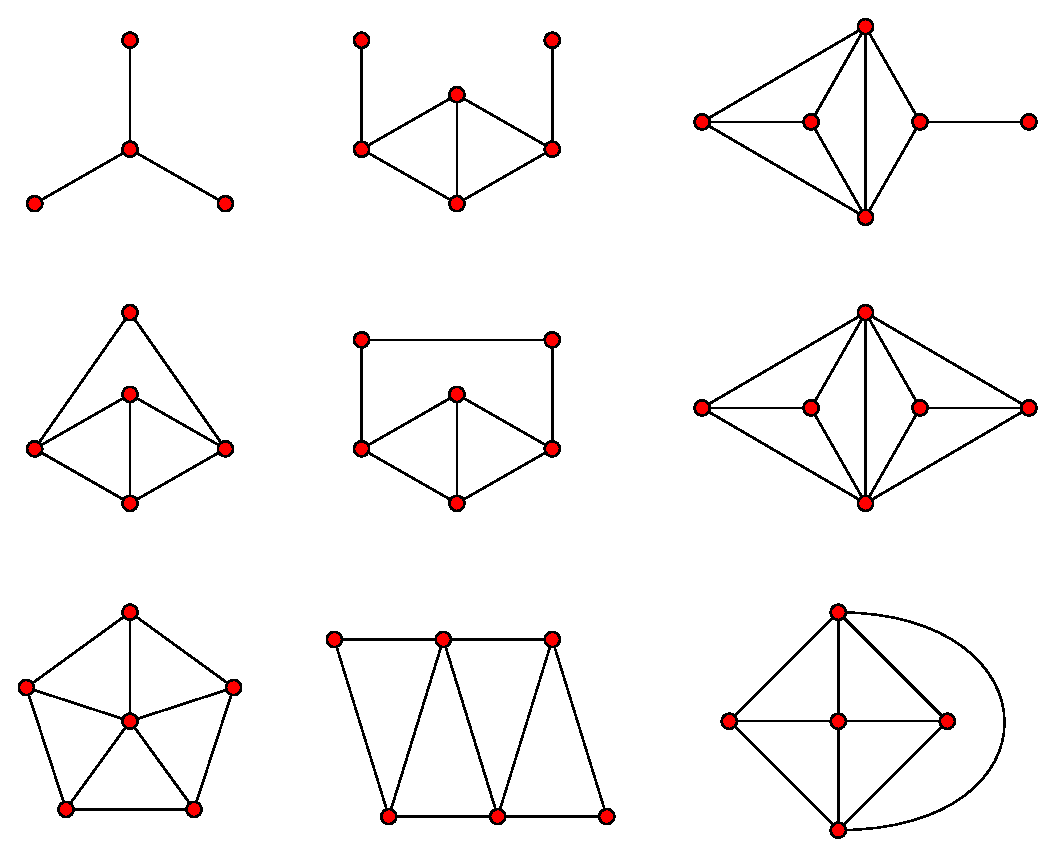
\includegraphics[width=\linewidth]{forbidden.eps}
	\caption{Zakazane grafy indukowane w grafie krawędziowym}
	\label{fig:forbidden}
\end{figure}

\section{Założenia programu}

\subsection{Dane wejściowe}

Wejściowy graf krawędziowy będzie można wczytać za pomocą macierzy sąsiedztwa lub listy sąsiedztwa. Wczytywanie może odbywać się z pliku, lub interaktywnie z poziomu aplikacji. Zaimplementowana zostanie możliwość zapisania stworzonego grafu do pliku. 
Wczytany graf będzie wizualizowany tak aby istniała możliwość zweryfikowania go przez użytkownika

\subsection{Działanie algorytmu}

Testy przedstawione w~poprzednim punkcie powinny zapewnić poprawność działania algorytmu.

\subsection{Wizualizacja działania algorytmu}

Program będzie musiał w sposób czytelny przedstawiać działanie zaimplementowanego algorytmu. Oznacza to że w każdym momencie powinno być dokładnie widoczne jaki krok jest obecnie wykonywany, którymi wierzchołkami i krawędziami manipulujemy, jaka jest postać grafu odtworzonego z~wczytanego grafu krawędziowego.
\bibliography{bibliografia} 
\bibliographystyle{plain}
\end{document}


